\documentclass{article}

\usepackage{pandekten}

\title{QED}
\author{Ch\=an Taku}

\begin{document}

\maketitle

\section{Gallery}

\subsection{Vertex Function}

\begin{proposition}{1-Loop Correction of Vertex Function}{1_loop_correction_of_vertex_function}
    \begin{center}
        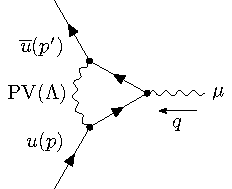
\includegraphics{img/vertex/vertex-1L.pdf}
    \end{center}
    \begin{align*}
        &= \frac{\alpha}{2\pi} \int_{[0,1]^3} \dd{x} \dd{y} \dd{z} \delta(x+y+z - 1) \\
        &\phantom{{}={}} \overline{u}(p')
        \left(
            \gamma^\mu\qty[\log \frac{z\Lambda^2}{\Delta} + \frac{1}{\Delta}\qty((1-x)(1-y)q^2 + (1-4z+z^2)m^2)] \vphantom{\frac{i\sigma^{\mu\nu}q_\nu}{2m}\qty[\frac{1}{\Delta}2m^2 z(1-z)]}
        \right. \\
        &\phantom{{}={}} \left.
        {} + {} \frac{i\sigma^{\mu\nu}q_\nu}{2m}\qty[\frac{1}{\Delta}2m^2 z(1-z)] \vphantom{\gamma^\mu\qty[\log \frac{z\Lambda^2}{\Delta} + \frac{1}{\Delta}\qty((1-x)(1-y)q^2 + (1-4z+z^2)m^2)]}
        \right)
        u(p),
    \end{align*}
    where
    \[ \Delta = -xyq^2 + (1-z)^2 m^2. \]
    Note that terms of $\bigO(\Lambda^{-1})$ are dropped.
\end{proposition}

\subsection{Electron Self-Energy}

\begin{proposition}{1-Loop 1PI of Electron}{1_loop_1pi_of_electron}
    \begin{center}
        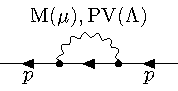
\includegraphics{img/electron/electron-1L.pdf}
    \end{center}
    \begin{align*}
        & -i\Sigma_2(p) \\ &= (-i)\frac{\alpha}{2\pi} \int_0^1 (2m_0 - x\slashed{p}) \log\qty(\frac{x\Lambda^2}{(1-x)m_0^2 + x\mu^2 - x(1-x)p^2}).
    \end{align*}
\end{proposition}

\subsection{Photon Self-Energy}

\begin{proposition}{1-Loop 1PI of Photon}{1_loop_1pi_of_photon}
    \begin{align*}
        &\phantom{{}={}} \qty(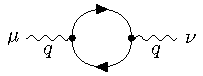
\includegraphics[valign=c]{img/photon/photon-1L.pdf})_{\operatorname{D}(d)} \\
        &= i\Pi_2^{\mu\nu}(q) = i(q^2 g^{\mu\nu} - q^\mu q^\nu) \Pi_2(q^2),
    \end{align*}
    where
    \[ \Pi_2(q^2) = \frac{-8e^2}{(4\pi)^{d/2}} \int_0^1 \dd{x} x(1-x) \frac{\Gamma(2-d/2)}{\Delta^{2-d/2}}, \]
    and
    \[ \Delta = m^2 - x(1-x)q^2. \]
    Let $\epsilon = 4-d$ and drop terms of $\bigO(\epsilon)$, we find
    \[ \Pi_2(q^2) = -\frac{2\alpha}{\pi} \int_0^1 \dd{x} x(1-x) \qty(\frac{2}{\epsilon} - \log \Delta - \gamma + \log(4\pi)). \]
\end{proposition}

% \bibliographystyle{plain}
% \bibliography{main}

\end{document}
